\pagebreak
\section{Experiment 3}
This experiment investigates the size of the test set and the reliability of a system given greater independence in datasets. This time the class means are defined in a similar manner to the process in Experiment 2, however the weighting differs as the error probability is given a wider allowable range of 1-10\%. Ten such test sets are created and stored independently, and the process once again iterates 10 times for each sample size $N_{D} = 5, 10, 20, 50$ and then intervals of 50 until $N_{D} = 500$. Once again, as in Experiment 2, the Test Set Error should converge to the true error, and the training set error should remain constant as the training set itself is never changed.

\subsection{Results and Discussion}
As expected the error converges to the true error and, as mentioned in Experiment 2, this occurs at $N_{D} > 200$ in the 5-dimensional space selected for this experiment. The oscillatory nature observed previously in Experiment 2 presents similar characteristics here as the standard deviation in error varies as seen in \ref{fig:Exp3}(b). So far this allows us to conclude that greater reliability in approximating the true error can be achieved with larger test data sets. However the standard deviation does not significantly reduce suggesting that an increase in test dataset may not be enough to improve reliability in the system - and that the increase in reliability is more prevalent when an increase in training data is offered (as in Experiment 1).

\begin{figure}[h]
	\centering
	\begin{subfigure}{.5\textwidth}
		\centering
		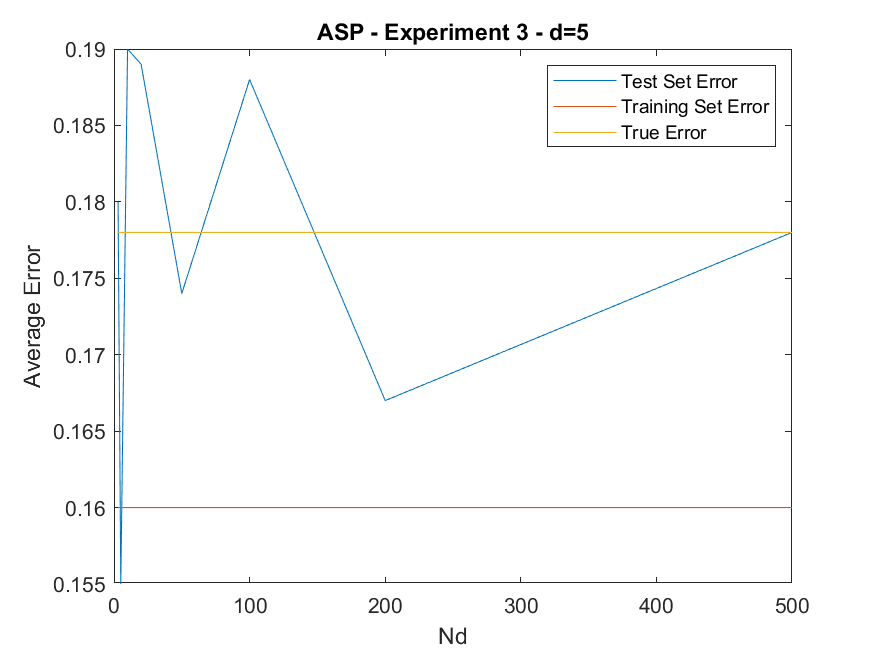
\includegraphics[width=.95\linewidth]{./code/Exp3-results/ErrorComparison_5.png}
		\caption{5 Dimensions}
	\end{subfigure}%
	\begin{subfigure}{.5\textwidth}
		\centering
		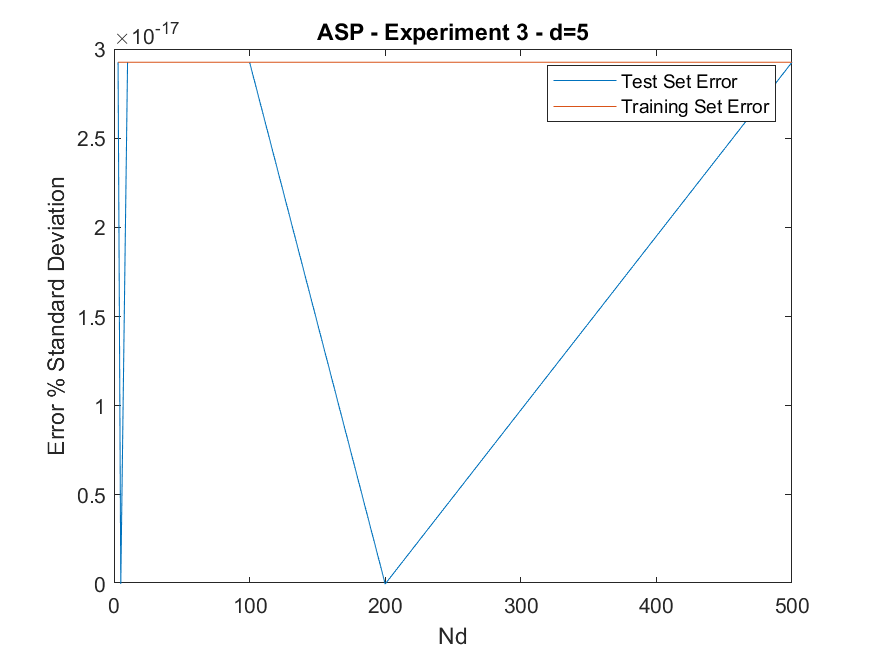
\includegraphics[width=.95\linewidth]{./code/Exp3-results/ErrorStandardDeviation_5.png}
		\caption{Standard Deviation of Error \% vs Test Set Size}
	\end{subfigure}
	\caption{Experiment 3 Results - Test Set Size Reliability}
	\label{fig:Exp3}
\end{figure}
